\section{Resultados y Análisis}

En esta sección se presentan los resultados obtenidos al resolver el Problema del Clique Máximo sobre la instancia \textit{keller4} del benchmark DIMACS \parencite{mascia_dimacs}, utilizando la formulación ILP descrita en la Sección~\ref{subsec:formulacion} implementada en Pyomo \parencite{pyomo2021} con el solver HiGHS \parencite{highs2024}.

\subsection{Descripción de la instancia}

La instancia \textit{keller4} pertenece a la familia Keller, basada en la conjetura de Keller sobre teselaciones del espacio mediante hipercubos \parencite{mascia_dimacs}. Sus características se resumen en la Tabla~\ref{tab:instancia}.

\begin{table}[H]
\centering
\caption{Características de la instancia keller4.}
\label{tab:instancia}
\begin{tabular}{lr}
\hline
\textbf{Propiedad} & \textbf{Valor} \\
\hline
Vértices ($|V|$) & 171 \\
Aristas ($|E|$) & 9\,435 \\
Densidad & 0.6491 \\
Clique máximo conocido ($\omega$) & 11 \\
Aristas del complemento ($|\bar{E}|$) & 5\,100 \\
\hline
\end{tabular}
\end{table}

\subsection{Dimensiones del modelo ILP}

El modelo formulado en Pyomo contiene 171 variables binarias de decisión (una por vértice) y 5\,100 restricciones de no-adyacencia, correspondientes a las aristas del grafo complemento $\bar{G}$. La razón de restricciones por variable es de 29{,}8, lo que indica un modelo fuertemente restringido.

\subsection{Resultados de la resolución exacta: comparativa de solvers}

Para evaluar el efecto del solver MIP en el tiempo de resolución, se ejecutó el mismo modelo ILP \emph{(Pyomo, idéntica formulación)} con dos solvers: HiGHS \parencite{highs2024} y GLPK. En GLPK se fijó un límite de tiempo de 300 segundos (5 minutos). Los resultados se resumen en la Tabla~\ref{tab:resultados}.

\begin{table}[H]
\centering
\caption{Comparativa de resolución del MCP sobre keller4: HiGHS vs GLPK.}
\label{tab:resultados}
\begin{tabular}{lrr}
\hline
\textbf{Métrica} & \textbf{HiGHS} & \textbf{GLPK} \\
\hline
Mejor solución encontrada ($\omega$) & 11 & 11 \\
Óptimo conocido & 11 & 11 \\
Tiempo de resolución & 12--18 s (según ejecución) & $> 300$ s (\textit{timeout}) \\
Estado del solver & Óptimo & Factible (sin probar optimalidad) \\
\hline
\end{tabular}
\end{table}

HiGHS resolvió el modelo hasta optimalidad en un tiempo de entre 12 y 18 segundos (dependiendo de la ejecución), alcanzando el óptimo conocido $\omega = 11$. GLPK, en cambio, encontró un clique factible del mismo tamaño pero no logró cerrar la brecha de optimalidad dentro del límite de 300 segundos, terminando con estado \textit{feasible}. Esto evidencia el impacto de las técnicas modernas de resolución MIP (planos de corte, heurísticas, preprocesamiento) implementadas en HiGHS frente a la base más austera de GLPK.

La solución fue validada verificando que el subgrafo inducido por los 11 vértices del clique es completo, es decir, contiene exactamente $\binom{11}{2} = 55$ aristas, todas presentes en el grafo original.

\subsection{Análisis de la relajación LP}

Para evaluar la calidad de la formulación, se resolvió la relajación lineal continua del modelo (reemplazando $x_i \in \{0,1\}$ por $x_i \in [0,1]$). Los resultados se presentan en la Tabla~\ref{tab:relajacion}.

\begin{table}[H]
\centering
\caption{Comparación entre solución entera y relajación LP.}
\label{tab:relajacion}
\begin{tabular}{lr}
\hline
\textbf{Métrica} & \textbf{Valor} \\
\hline
Cota LP (relajación) & 85.50 \\
Solución entera (ILP) & 11 \\
Brecha de integralidad & 87.1\% \\
\hline
\end{tabular}
\end{table}

La brecha de integralidad de 87.1\% indica que la relajación LP proporciona una cota superior muy débil para esta instancia. Este fenómeno es bien conocido en la literatura: la formulación estándar del MCP basada en restricciones de pares no adyacentes produce relajaciones LP intrínsecamente débiles, especialmente en grafos con estructura regular \parencite{bomze1999, nemhauser1988}. Esto implica que el solver debe explorar un árbol de Branch \& Bound extenso para cerrar la brecha entre la cota LP y la solución entera óptima.

\subsection{Visualización}

La Figura~\ref{fig:clique_resultado} muestra el grafo keller4 con el clique máximo destacado en rojo. Los vértices pertenecientes al clique se identifican con mayor tamaño y las aristas entre ellos se resaltan. La distribución de grados del grafo muestra que los vértices del clique poseen grados superiores al promedio, lo cual es consistente con la estructura esperada de un clique en un grafo denso.

\begin{figure}[ht]
\centering
% Imagen generada por el notebook: grafo_clique.png
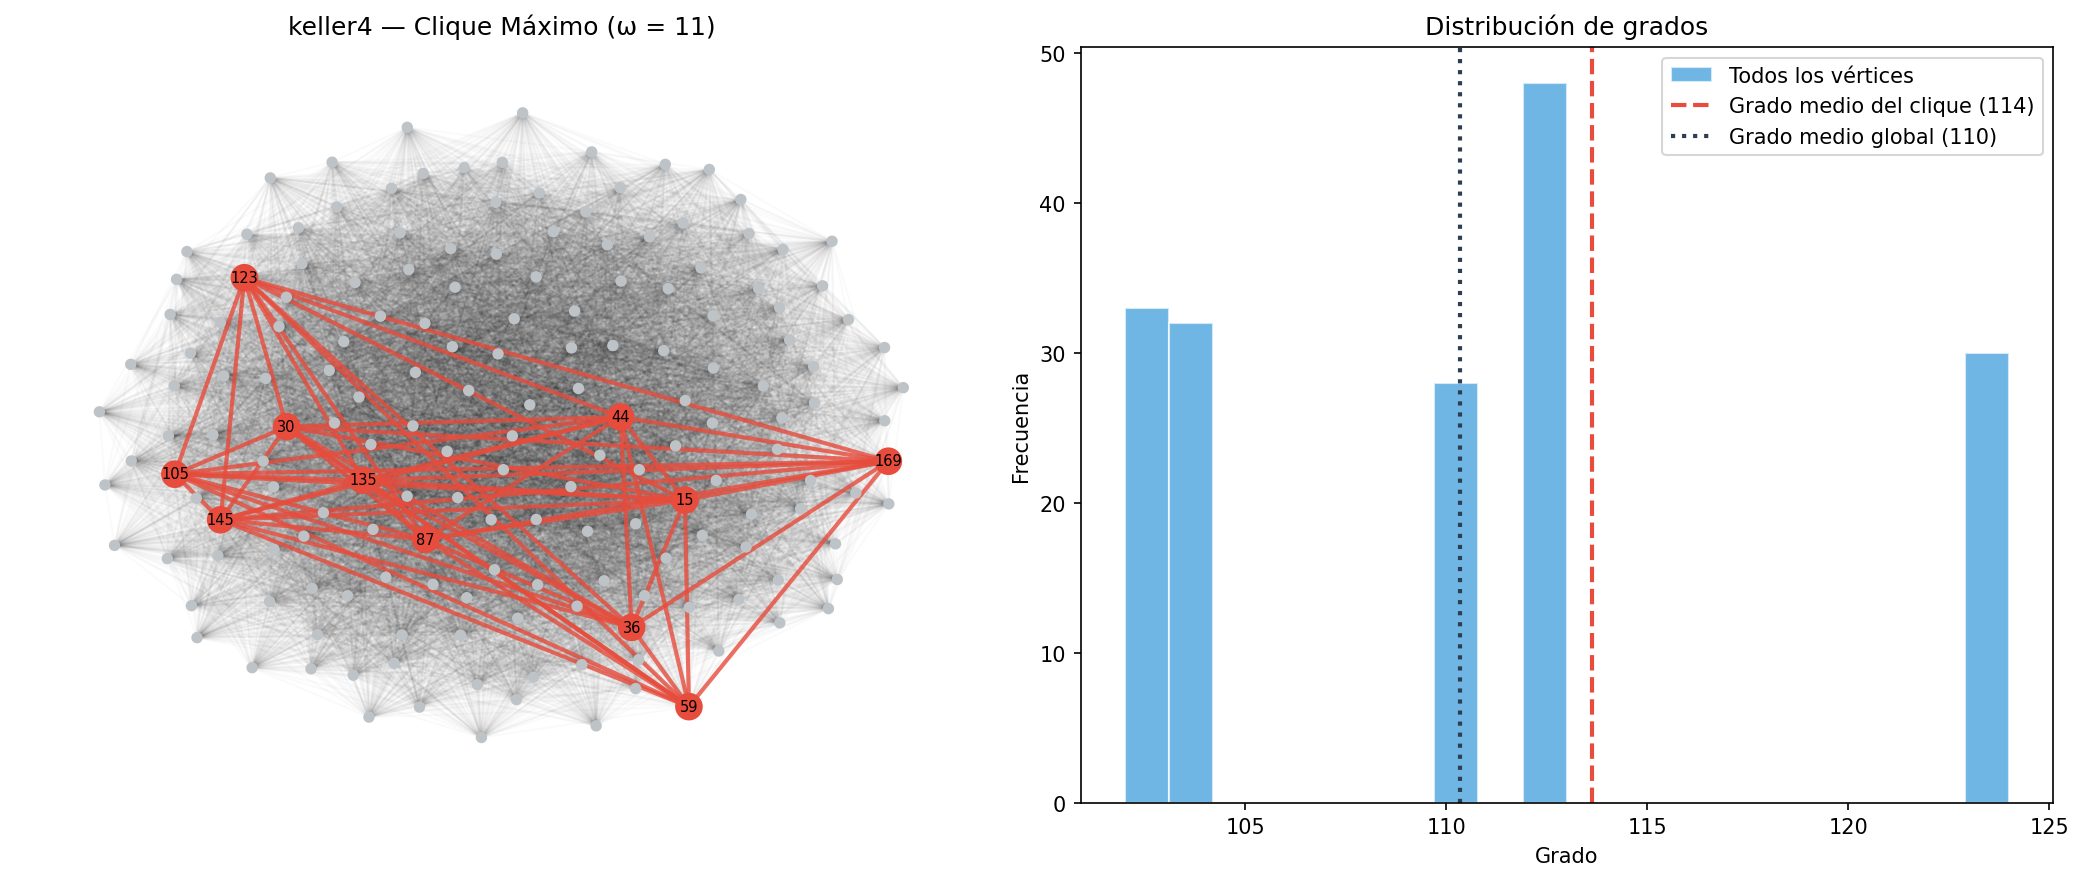
\includegraphics[width=0.75\textwidth]{../notebook/resultados_keller4_pyomo.png}
\caption{Grafo keller4 con el clique máximo resaltado (vértices del clique en rojo y mayor tamaño).}
\label{fig:clique_resultado}
\end{figure}
